\documentclass{evolang12}
\usepackage{graphicx}
\usepackage{url}
\usepackage{authblk}
\usepackage{floatrow}

\begin{document}

\title{Learning to communicate \\ about conceptual hierarchies}
\author[1*]{ANONYMOUS AUTHOR 1}
\author[1]{ANONYMOUS AUTHOR 2} 
\author[2]{ANONYMOUS AUTHOR 3}
\author[3]{ANONYMOUS AUTHOR 4}
\affil[*]{Corresponding Author: name@domain.com}
\affil[1]{This Department, University X, City, Country}
\affil[2]{That Department, University Y, City, Country}
\affil[3]{Other Department, University Z, City, Country}

%%%%% INSTRUCTIONS FOR ADDING AUTHORS %%%%%

%Initial submissions should be anonymous - DO NOT INCLUDE ANY IDENTIFYING INFORMAITON IN THE SUBMISSION VERSION -(i.e., no author details should be added above). To avoid problems with page limits, please include the appropriate number of placeholders for authors. If multiple authors share an affiliation, they can be paired with the appropriate affiliation using the numbers in the square brackets next to "author" and "affil" to save space. Designate a single corresponding author using the asterisk.

\maketitle

%% Introduce problem
Natural languages provide speakers with remarkable flexibility in the labels they may use to refer to things. In addition to the combinatorial explosion of modifiers afforded by compositionality \cite{Partee95_LexicalSemanticsCompositionality,WintersKirbySmith14_LanguagesAdapt}, we have a number of lexicalized nominal terms at our disposal. \emph{Dalmatian}, \emph{dog}, and \emph{animal} can all truthfully be used to talk about the same Dalmatian at different levels of specificity, with one level of the conceptual hierarchy -- the basic-level -- privileged over the others \cite{RoschMervisGray___BoyesBraem76_BasicObjects}. Recent work on the pragmatics of nominal reference has explained preferences for different labels in different context using a computational model that captures informativeness and production cost \cite<e.g.>{GrafEtAl16_BasicLevel}. But there remains a more fundamental evolutionary question: why do multiple levels of reference coexist in the lexicon instead of a simpler system only containing subordinate terms? 

%% Introduce hypothesis & interactive paradigm
Our hypothesis, motivated both by classic work on concept representations and contemporary work on the selective pressures induced by communication, is that lexicalization of conceptual hierarchies is a function of (1) the structure and statistics of entities in the environment, and (2) the particular contexts in which communication occurs. In particular, we expect hierarchical lexica to form when features can be encoded as predictable clusters and communicative goals require distinctions to be drawn at multiple levels. To test this hypothesis, we designed a repeated reference game in which pairs of participants interactively created an artificial language to communicate with each other about objects in context. 

%% Introduce task 
In this game, participants were paired over the web and placed in a shared environment containing a grid of four objects (Fig. 1A) and a `chatbox' to send messages from a pre-specified vocabulary of sixteen words (Fig. 1B). On each of ninety trials, one player --- the `speaker' --- was privately shown a highlighted target object and allowed to send a single word to help their partner select this object from the array of distractors. The set of objects was designed to cluster in a natural hierarchy (Fig. 1C) so that distractors may belong to the target's superordinate-level category (defined by shape), basic-level category (defined by color/texture), or neither, thus creating three kinds of contexts. In addition to fine-grained behavioral trajectories observed over the course of the game, we conducted a post-test to explicitly probe players' lexica. For each word, we asked players to select all objects to which that word applies, allowing us to distinguish between subordinate terms that apply to only one element and basic-level terms that apply to all elements belonging to an intermediate level of the hierarchy: striped circles, for example. %Players were awarded bonuses for correct responses and switched roles on each round; neither player was trained on word-object mappings in advance, so all meanings had to be created over the course of interaction. 

%% Introduce manipulations & summarize results
%% suggest interpretation (i.e. path-dependence?) and speculate about set-based version & model?
We manipulated the statistics of the context in a between-subjects design to test the contribution of communicative relevance to lexicalization. In the critical `uniform' condition, all three kinds of context were equally likely, thus providing high diversity in the relevant distinctions that must be drawn. We also ran three control conditions in which a single kind of context dominated, e.g. in the `subordinate-required' condition, the majority of trials contained distractors that belonged to the same basic-level as the target (e.g. Fig. 1A), theoretically requiring speakers to lexicalize a label for each target. We counted the relative number of subordinate-level terms and basic-level terms in the post-test and found that the uniform condition was more likely to gave rise to lexica in which multiple levels of reference coexist. This suggests that pragmatic pressures for informativity in a diversity of communicative contexts is instrumental for the lexicalization of hierarchical nominal reference systems. Our independent minds organize the world into conceptual hierarchies but our shared language only evolves to reflect this structure when it is communicatively relevant. 

\begin{figure}[t]
\begin{center}
{\caption{{\footnotesize (A) Example array of elements the matcher must choose from. The target is highlighted for the speaker with a black square. In this \emph{subordinate-required} trial there is a distractor at the same basic-level (striped texture) as the target, so using a basic-level label would be insufficient. (B) Chat box interface. (C) Hierarchical organization of stimuli.  \label{exp}}}}
{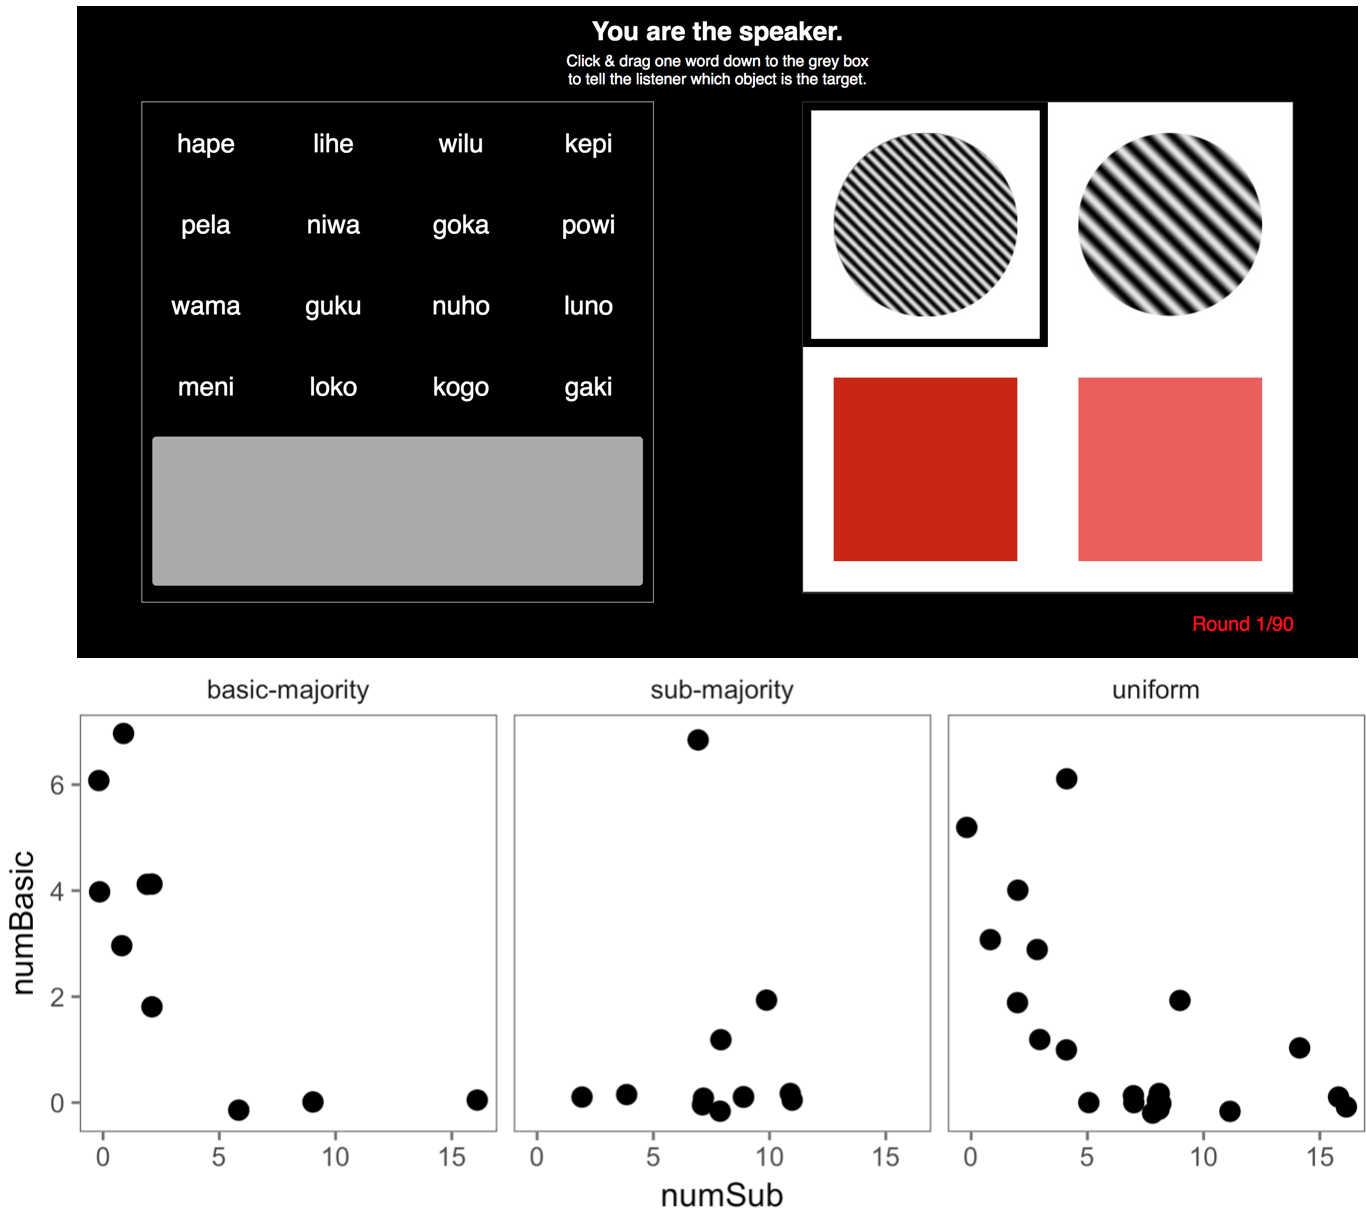
\includegraphics[scale=.41]{fig.png}}
\end{center}
\end{figure}

\newpage

\bibliographystyle{apacite}
\bibliography{evolang} 

\end{document}
